\section{Feasibility Study}
\label{sec:study}
\amirian{How about Covert Channel throughput as an alternative title?}
%Our goal in developing this technique is to demonstrate how easy it is for
%attackers to exploit the pervasive memory bus covert channel and obtain
%co-residency information, thereby motivating the need to address it. This
%information can be used by attackers in aiding a lot of attack scenarios
%\todo{for example?} or simply learn the internal mechanisms of a cloud. 
%In the section, we explore some ways in
%which the tool can be used to gain some insights into lambda activity in some
%AWS regions.  

\ins{In this section, we present various measurements to demonstrate the 
practicality of covert channel with lambdas using the co-residence detector.
As already discussed in section \todo{3?}, the amount of information that 
can be transferred depends on the number of rendezvous points (co-resident 
clusters of lambdas) that materialize during the attack and channel capacity 
per each rendezvous point. We first get an estimate on the 
capacity of the covert channels established at these rendezvous points. 
Later, we perform a study on the colocation 
density in various AWS regions to understand the number of rendezvous points
and factors that affect it.}

\subsection{Datarate per rendezvous}


\begin{figure}[!t]
  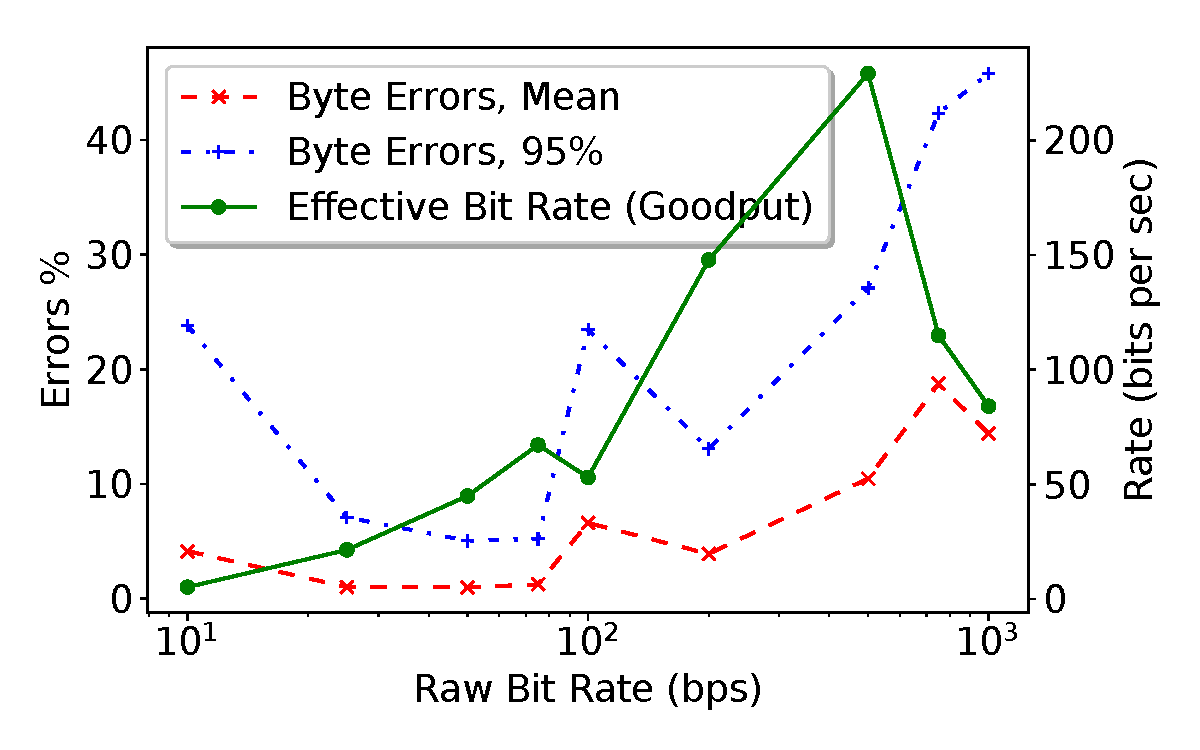
\includegraphics[width=.99\linewidth]{fig/channel_rate_3gb.pdf}
  \caption{\todo{increase font}
\label{fig:channel}}
\end{figure}


\ins{Once co-residence between any two lambas is established, the attacker can then use 
the same memory bus hardware to perform covert communication. Wu et al.~\cite{wuusenix2012}
that first introduced covert channel based on this hardware also presented an efficient 
and error-free communication protocol targeting cloud-based platforms like VMs.
While such advanced protocol should theoretically work for lambdas as well, extending 
it is beyond the scope of this work. We do, however, use a much simpler albeit 
inefficient protocol to report a conservative estimate of the capacity of each 
covert channel.}

\ins{Our protocol for data transfer uses the same mechanisms we used for co-residence detection in 
section \todo{ref 5.2} to send and receive bits, and perform 
clock synchronization. The only difference is that since we now only expect just the 
sender and receiver lambdas to be active (i.e., although there may be tens of other co-resident 
lambdas, we can use our co-residence detector to identify every lambda and set others 
inactive), we don't need to worry about noise from multiple receivers, the result 
being receiver can sample continously (\todo{ref 5.2.2}) and time spent for each bit can be 
extremely small (in the order of milliseconds instead of seconds). Naturally, we want 
this time to be as small as possible to increase bitrate, however, the chances of 
erasures (errors) increase too as both sender and receiver may get descheduled during this time.
To demonstrate this, we launch hundreds of (3 GB) lambdas on AWS and use our co-residence detector to 
establish tens of covert channels. We then send data over these channels at various bitrates 
and record the error ratio (for byte-sized data segments). Figure~\ref{fig:channel} shows 
the mean error ratio at 50\% and 95\% confidence, both of which increase with the bitrate.}

\ins{To correct these errors, we can use block-based error correction codes like Reed-Solomon with 
byte-sized symbols\cite{wuusenix2012} (as descheduling may result in burst errors). However, error 
correction comes with an overhead; Reed-Solomon requires twice as many extra symbols as there are errors
to correct. So, for each bitrate, we compute effective bitrate by substracting the overhead of error 
correction symbols required to correct its corresponding 95\% error. From Figure~\ref{fig:channel},
we can see that effective bitrate rises to a maximum of over 200 bps (at 500bps raw rate) before 
falling again due to high error rate. 
We confirmed this by sending Reed-Solomon encoded data over the covert channels at this rate and observed 
near-zero data corruption. Thus, we conclude that, by a conservative estimate, we can safely send data 
across each of these covert channels at a significant rate of ~200 bps.}


\subsection{Rendezvous density}
\todo{Changes due to above subsection}
In this section, we present a variety of measurements on serverless function
density on AWS using our co-residence detector, and the factors that may affect
this density. As we discussed earlier, the key challenge in enabling traditional
covert channels on the cloud is placingthe sender and receiver on the same
machine. So we attempt to answer the following question: Assuming that the user
launches a number of (sender and receiver) lambdas at a specific point in time,
what is the expected number of such co-resident pairs that they might see? We
deploy a large number of lambdas on various AWS regions and report the
co-residence density -- that is, the average number of lambdas that end up
co-resident on each server.  The higher the co-residence density, the easier it
is for the user to ultimately establish covert channels with lambdas. Unless
specified otherwise, all the experiments are performed with 1.5 GB lambdas and
executed successfully with \textbf{zero error} in co-residence detection.


\begin{figure*}[!t]
    \begin{subfigure}{.5\textwidth}
      \centering
      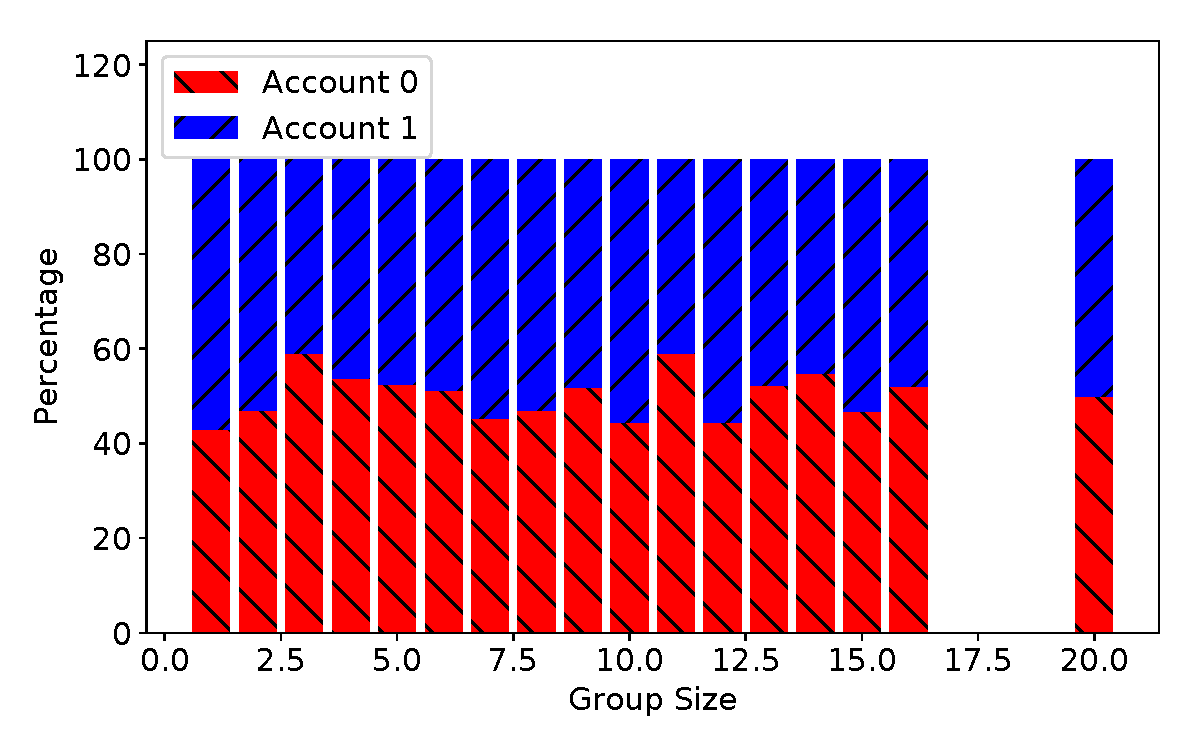
\includegraphics[width=.99\linewidth]{fig/different-accounts.pdf}
    %   \caption{1a}
    %   \label{fig:sfig1}
    \end{subfigure}%
    \begin{subfigure}{.5\textwidth}
      \centering
      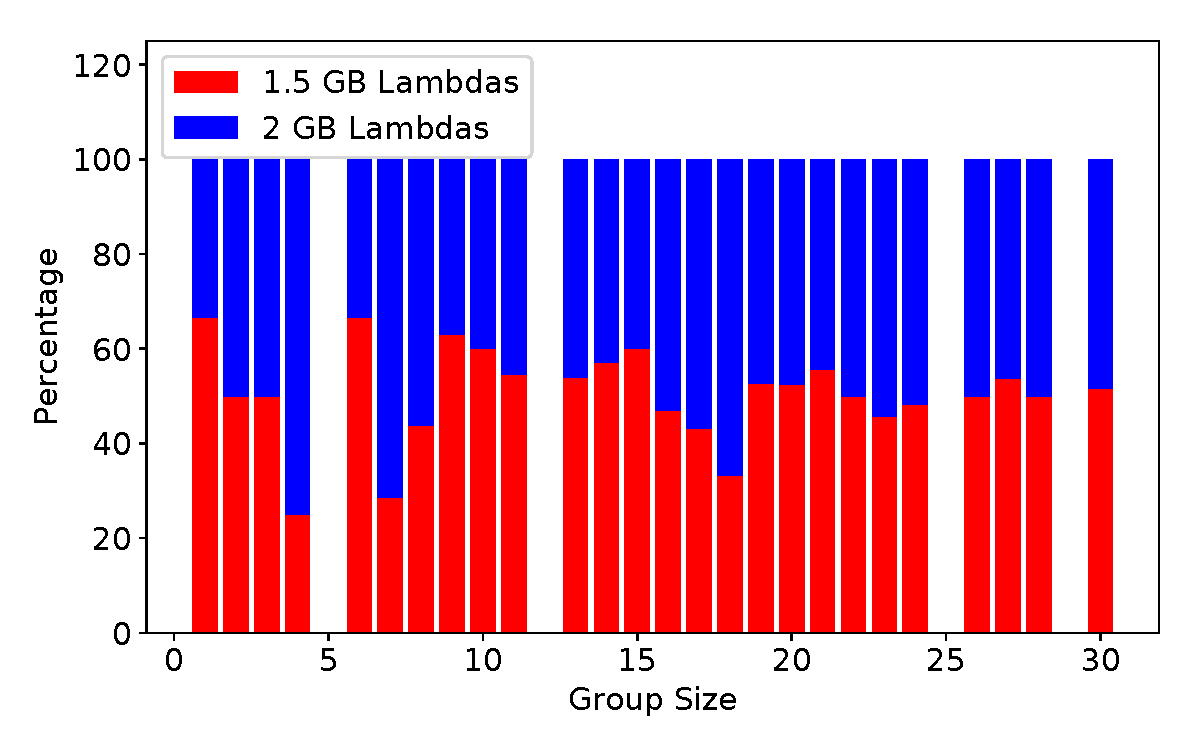
\includegraphics[width=.99\linewidth]{fig/different-sizes.pdf}
    %   \caption{1b}
    %   \label{fig:sfig2}
    \end{subfigure}

    \caption{The left plot shows the breakdown of co-resident groups (of varying
    sizes) of lambdas by two different accounts in an experiment of 1000
    lambdas, where 500 lambdas are launched from each account. The uniformity of
    the split indicates that the lambda scheduler might be invariant to the
    account the lambdas are launched from. Similar results are shown for
    different lambda sizes in the right plot. }
    \label{fig:factors}
\end{figure*}


\subsubsection{Across AWS regions}
\todo{clarify the attacker model here, per R1 comments}
We execute our co-residence detector with 1000 1.5 GB Lambdas in various AWS
regions. Figure~\ref{fig:awsregions} comprises multiple plots depicting
the co-resident groups per region, with each bar indicating the fraction of
lambdas that detected a certain number of neighbors (i.e., that belong to a
co-resident group of a certain size). Plots that skew to the right indicate a
higher co-residence density when compared to the plots skewed to the left (also
illustrated in Figure~\ref{fig:density}). We note that, in most regions, almost
all lambdas recognize at least one neighbor (indicated by smaller or
non-existent first bar in each plot). We hypothesize that the co-residence
density is (inversely) dependent on the total number of servers and the lambda
activity in the region, both of which can be assumed to be lower in newer AWS
regions, hence the higher co-residence density in those regions as we can see in
Figure~\ref{fig:density}. The ample co-residence in general across all the
regions shows that lambdas provide a fertile ground for covert channel attacks.
%We note that the largest co-resident group on a single machine was comprised of 25 lambdas. 


\subsubsection{Other factors}
We also examine how co-residence is affected by various launch strategies that
the user may use, like deploying lambdas from multiple AWS accounts and
different lambda sizes. In particular, we wish to determine if we our mechanism
exhibits different results when: 1) the user deploys sender lambdas and receiver
lambdas on two separate accounts (normally the case with covert channels) and 2)
the senders and receivers are created with different lambdas sizes.  To answer
these questions, we run an experiment with 1000 lambdas of which we launch 500
lambdas from one account (senders) and 500 from other deployed in a random
order. The co-residence observed was comparable to the case where all the
lambdas were launched from one account. In the left subfigure of
Figure~\ref{fig:factors}, we show the breakdown of co-resident group of lambdas
of each size among the two accounts.  We can see that among the co-resident
groups of all sizes, roughly half of lambdas came from either account. This show
that lambda scheduler is agnostic to the accounts the lambdas were launched
from. We see similar results for different lambda sizes, as shown in the right
subfigure of Figure~\ref{fig:factors}.

%From our experiments, we also observe that co-residence density in a region
%barely changes during course of the day or the week (data not shown
%in any figure \todo{is this okay?}).  This gives the user the freedom to utilize this
%technique at any time and expect similar results.
